\documentclass[a4paper,10pt]{article}
\usepackage[utf8]{inputenc}
\usepackage[spanish]{babel}
\usepackage[affil-it]{authblk}
\usepackage{enumerate}
\usepackage{graphicx}
\usepackage{hyperref}
\usepackage{amsmath}
\usepackage{amssymb}
\usepackage{cancel}
\usepackage{tikz}
\usepackage{float}
\usepackage{cleveref}
\usepackage[margin=1.4in]{geometry}
\usepackage[labelfont=bf]{caption}
\usetikzlibrary{calc}
\numberwithin{equation}{section}

%Indentation
\setlength{\parindent}{0ex}

%Multiple References

\usepackage{xparse}
\ExplSyntaxOn
\NewDocumentCommand{\mref}{m}{\quinn_mref:n {#1}}
\seq_new:N \l_quinn_mref_seq
\cs_new:Npn \quinn_mref:n #1
 {
  \seq_set_split:Nnn \l_quinn_mref_seq { , } { #1 }
  \seq_pop_right:NN \l_quinn_mref_seq \l_tmpa_tl
  ( % print the left parenthesis
  \seq_map_inline:Nn \l_quinn_mref_seq
    { \ref{##1},\nobreakspace } % print the first references
  \exp_args:NV \ref \l_tmpa_tl 
  ) 
 }
\ExplSyntaxOff


%Boxes

\newcommand*{\boxcolor}{blue}
\makeatletter
\renewcommand{\boxed}[1]{\textcolor{\boxcolor}{%
\tikz[baseline={([yshift=-1ex]current bounding box.center)}] \node [rectangle, minimum width=1ex,rounded corners,draw] {\normalcolor\m@th$\displaystyle#1$};}}
 \makeatother

%Constantes
\newcommand{\euler}{\mathrm{e}}
\newcommand{\im}{i}

%Lemas, teoremas, definiciones y pruebas
\newcommand{\definicion}{\textbf{Definición: }}
\newcommand{\lema}{\textbf{Lema: }}
\newcommand{\teorema}{\textbf{Teorema: }}
\newcommand{\prueba}{\textbf{Prueba: }}


%opening
\title{Mecánica Clásica Tarea \# 4}
\author{Favio Vázquez\thanks{Correo: favio.vazquezp@gmail.com}}\affil{Instituto de Ciencias Nucleares. Universidad Nacional Autónoma de México.}
\date{}

\begin{document}

\makeatletter
\def\@maketitle{%
  \newpage
  \null
  \vskip 2em%
  \begin{center}%
  \let \footnote \thanks
    {\Large\bfseries \@title \par}%
    \vskip 1.5em%
    {\normalsize
      \lineskip .5em%
      \begin{tabular}[t]{c}%
        \@author
      \end{tabular}\par}%
    \vskip 1em%
    {\normalsize \@date}%
  \end{center}%
  \par
  \vskip 1.5em}
\makeatother

\maketitle

\section{Problema 1}

Una partícula de masa $m_1$ se mueve a lo largo de una recta, otra de masa $m_2$ lo 
hace a lo largo de otra reta perpendicular a la primera. Las partículas interaccionan 
entre sí por medio de la gravedad. Encuentra las ecuaciones de movimiento. Usando 
una computadora trace una trayectoria en el espacio de configuración para algunas 
masas y condiciones iniciales.

\vspace{.3cm}

Suponga que $m_2=m_1+\epsilon$, donde $\epsilon$ es una cantidad pequeña. Encuentre 
las ecuaciones de movimiento a primer orden en $\epsilon$. Usando una computadora 
trace una órbita genérica para este caso.

\vspace{.3cm}

\underline{Solución:} \vspace{.3cm}


\section{Problema 2}

Encuentre las ecuaciones de movimiento del péndulo doble usando únicamente métodos 
vectoriales. El péndulo doble tiene las dos masas iguales y las dos longitudes iguales.
Usando una computadora trace la trayectoria $(\theta_1$ vs $\theta_2)$ cuando las 
condiciones iniciales son

\begin{align*}
 \theta_1 &= \frac{\pi}{2} \\
 \theta_2 &= \pi \\
 \dot{\theta_1} &= 0 \\
 \dot{\theta_2} &= 0 
\end{align*}

\vspace{.3cm}

\underline{Solución:} \vspace{.3cm}

En la figura de abajo se muestra un diagrama del problema, 

\begin{figure}[H]
\center
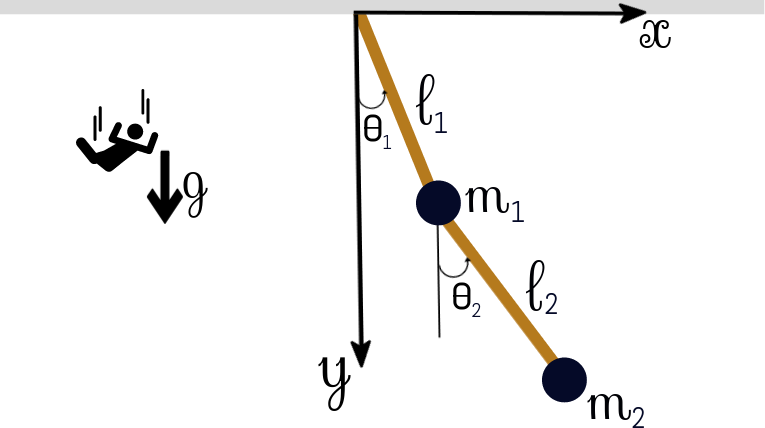
\includegraphics[scale=0.4]{problema2fig1}
\caption{Péndulo doble. Como muestra el muñequito la gravedad va dirigida hacia 
abajo.}
\label{fig:problema2fig1}
\end{figure}


Consideraremos un caso general en el cual las longitudes y masas pueden ser diferentes,
y luego haremos la simplificación que el enunciado indica. El doble péndulo consiste 
en dos masa $m_1$ y $m_2$ conectadas por barras sin masa de longitudes $l_1$ y $l_2$,
sujetas a la fuerza de gravedad, y constreñidas por las junturas entre las varas
a moverse en un plano. Escogeremos un sistema de coordenadas con el origen en el 
tope del punto de suspensión, y el eje $x$ como un eje horizontal en el plano del 
movimiento, y el eje $y$ hacia abajo, de manera tal que las fuerzas de gravedad 
tengan componentes positivas.

\vspace{.3cm}

El sistema tiene dos partículas, digamos que con posiciones $\mathbf{r_1}$ y $\mathbf{r_2}$,
cada una con componentes $(x_i,y_i,z_i)$. Como hemos dicho el sistema se moverá 
en el plano de $x-y$, por lo tanto consideraremos esto como una restricción, ligadura,
o constricción; entonces habrá una de estas constricciones para cada partícula, y 
hay otras dos más, el hecho de que cada barra tiene una longitud constante. Podemos 
escribir estas constricciones como:

\begin{align}
 z_1 &= 0, \\
 z_2 &= 0, \\
 |\mathbf{r_1}| &= l_1, \\
 |\mathbf{r_2} - \mathbf{r_1}| &= l_2.
 \label{eq:pendu1}
\end{align}

Entonces para el caso que consideremos del péndulo doble, tendremos solamente, dos (2)
grados de libertad, debido a que los originales seis (6) se reducen por las cuatro (4)
constricciones al movimiento que consideramos. 

\vspace{.3cm}

El lector familiarizado con este problema, ya clásico de la mecánica, recordará que en 
la formulación lagrangiana de este problema, las coordenadas generalizadas más utilizadas
y que simplifican la solución del problema son $\theta_1$ y $\theta_2$, por lo tanto
las ecuaciones de movimiento se expresarán en término de las mismas, para así poder tener 
una comparación directa con el análisis vectorial del problema que haremos, con el escalar
que se trabaja en la formulación lagrangiana. Podemos encontrar expresiones para $\mathbf{r_1}$ y $\mathbf{r_2}$ en términos 
de los dos ángulos $\theta_1$ y $\theta_2$:

\begin{align}
 \mathbf{r_1} &= l_1\sen{\theta_1} + l_1\cos{\theta_1}
 \mathbf{r_2} &= \mathbf{r_1} +  l_2\sen{\theta_2} + l_2\cos{\theta_2}
 \label{eq:pendu2}
\end{align}

Ahora podemos encontrar los vectores de velocidad y aceleración en término de $\theta_1$ y $\theta_2$,
para $m_1$,

\begin{equation}
 \dot{\mathbf{r_1}} = \mathbf{v_1} = l_1 \dot{\theta_1} \cos{\theta_1} - l_1 \dot{\theta_1} \sen{\theta_1} = l_1 \dot{\theta_1}(\cos{\theta_1} - \sen{\theta_1}),
 \label{eq:pendu3}
\end{equation}

\begin{align}
\begin{split}
 \ddot{\mathbf{r_1}} = \mathbf{a_1} &= l_1 \ddot{\theta_1} \cos{\theta_1} - l_1 \dot{\theta_1}^2 \sen{\theta_1} - l_1 \ddot{\theta_1} \sen{\theta_1} - l_1 \dot{\theta_1}^2 \cos{\theta_1}, \\
 &=  l_1 \ddot{\theta_1} (\cos{\theta_1} - \sen{\theta_1}) - l_1 \dot{\theta_1}^2 (\cos{\theta_1} +  \sen{\theta_1}),
 \label{eq:pendu4}
\end{split}
\end{align}

y para $m_2$

\begin{equation}
 \dot{\mathbf{r_2}} = \mathbf{v_2} = \mathbf{v_1} + l_2 \dot{\theta_2} \cos{\theta_2} - l_2 \dot{\theta_2} \sen{\theta_2} = l_2 \dot{\theta_2}(\cos{\theta_2} - \sen{\theta_2}),
 \label{eq:pendu5}
\end{equation}

\begin{align}
\begin{split}
 \ddot{\mathbf{r_1}} = \mathbf{a_2} &= \mathbf{a_1} + l_2 \ddot{\theta_2} \cos{\theta_2} - l_2 \dot{\theta_2}^2 \sen{\theta_2} - l_1 \ddot{\theta_2} \sen{\theta_2} - l_2 \dot{\theta_2}^2 \cos{\theta_2}, \\
 &= \mathbf{a_1} + l_2 \ddot{\theta_2} (\cos{\theta_2} - \sen{\theta_2}) - l_2 \dot{\theta_1}^2 (\cos{\theta_2} +  \sen{\theta_2}),
 \label{eq:pendu6}
\end{split}
\end{align}

Para poder construir las ecuaciones de movimiento en la metodología vectorial necesitamos 
conocer el sentido, dirección y magnitud de las fuerzas que actúan sobre las partículas 
en consideración. En este caso las fuerzas que actúan para $m_1$ son la tensión de las 
dos cuerdas (que llamaremos $\mathbf{T_1}$ y $\mathbf{T_2}$ respectivamente), y la gravedad.
La tensión de la cuerda $l_1$, sobre $m_1$ actúa lo largo de $-\mathbf{r_1}$, y la tensión 
de la cuerda $l_2$ actúa a lo largo de ($\mathbf{r_2} - \mathbf{r_1}$), entonces podemos 
escribir la fuerza $\mathbf{F_1}$ como

\begin{equation}
 \mathbf{F_1} = T_1 \frac{-\mathbf{r_1}}{|\mathbf{r_1}|} + T_2 \frac{\mathbf{r_2} - \mathbf{r_1}}{|\mathbf{r_2} -\mathbf{r_1}|}
	      + m_1 \mathbf{g} = - \frac{T_1}{l_1} \mathbf{r_1} + \frac{T_1}{l_1} (\mathbf{r_2} - \mathbf{r_1}) + m_1 \mathbf{g}.
\end{equation}

Las fuerzas sobre $m_2$ son la tensión de la cuerda $l_2$ a lo largo de -($\mathbf{r_2} - \mathbf{r_1}$)
y la gravedad,

\begin{equation}
 \mathbf{F_2} = T_2 \frac{-(\mathbf{r_2} - \mathbf{r_1})}{|\mathbf{r_2} -\mathbf{r_1}|}
	      + m_2 \mathbf{g} = - \frac{T_2}{l_2} (\mathbf{r_2} -\mathbf{r_1}) + m_2 \mathbf{g}.
\end{equation}

Estamos ahora en posición para escribir las ecuaciones de movimiento para el péndulo 
doble utilizando la segunda ley de Newton en cada partícula, $\mathbf{F_i} = m_i \ddot{\mathbf{r_i}}$:

\begin{align}
 m_1 \ddot{\mathbf{r_1}} &= - \frac{T_1}{l_1} \mathbf{r_1} + \frac{T_1}{l_1} (\mathbf{r_2} - \mathbf{r_1}) + m_1 \mathbf{g}, \\
 m_2 \ddot{\mathbf{r_2}} &= - \frac{T_2}{l_2} (\mathbf{r_2} -\mathbf{r_1}) + m_2 \mathbf{g}.
\end{align}

Estas ecuaciones no son muy esclarecedoras del problema al cual nos enfrentamos, y ahora 
es claro por qué debemos expresar las mismas para $\theta_1$ y $\theta_2$, debido que como 
veremos estas se convertirán en cuatro ecuaciones diferenciales para cuatro incógnitas, 
$\theta_1$, $\theta_2$, $T_1$ y $T_2$. Escribimos entonces las ecuaciones de movimiento 
para las dos partículas en sus componentes en el plano\footnote{Acá utilizaremos la muy conocida separación
de componentes de fuerzas de la mecánica newtoniana} ($x-y$), utilizando (\ref{eq:pendu3}) y (\ref{eq:pendu4}) y 
la figura (\ref{fig:problema2fig1}),

Para $m_1$,

\begin{align}
 m_1 l_1 (\ddot{\theta_1}\cos{\theta_1} - \dot{\theta_1}^2\sen{\theta_1}) &= - T_1 \sen{\theta_1} + T_2 \sen{\theta_2}, \\
 -m_1 l_1 (\ddot{\theta_1}\sen{\theta_1} + \dot{\theta_1}^2\cos{\theta_1}) &= - T_1 \cos{\theta_1} + T_2 \cos{\theta_2} + m_1 g.
\end{align}

Para $m_2$,

\begin{align}
 m_2(l_1\ddot{\theta_1}\cos{\theta_1} - l_1\dot{\theta_1}^2\sen{\theta_1} + l_2\ddot{\theta_2}\cos{\theta_2} - l_2\dot{\theta_2}^2\sen{\theta_2})
 &= - T_2 \sen{\theta_2}, \\
 - m_2(l_1\ddot{\theta_1}\sen{\theta_1} + l_1\dot{\theta_1}^2\cos{\theta_1} + l_2\ddot{\theta_2}\sen{\theta_2} - l_2\dot{\theta_2}^2\cos{\theta_2})
 &= - T_2 \cos{\theta_2} + m_2 g.
\end{align}

Haciendo uso de algunas identidades trigonométricas como $\cos^2{\theta} +  \sen^2{\theta} = 1$, y
$\sen{\theta_2}\cos{\theta_1} - \cos{\theta_2}\sen{\theta_1} = \sen{(\theta_2 - \theta_1)}$, 
y un largo trabajo algebraico que no aportaría nada colocarlo explícitamente en esta tarea,
llegamos a que las ecuaciones de movimiento pueden escribirse como:

\begin{align}
 l_1\ddot{\theta_1} &= \frac{T_2}{m_1}\sen{\theta_2 - \theta_1} - g \sen{\theta_1}, \\
 l_1\dot{\theta_1}^2 &= \frac{T_1}{m_1} - \frac{T_2}{m_1}\cos{\theta_2 - \theta_1} - g \cos{\theta_1}, \\
 l_2\ddot{\theta_2} &= - \frac{T_2}{m_1}\sen{\theta_2 - \theta_1}, \\
 l_2\dot{\theta_2}^2 &= \frac{T_2}{m_2} - \frac{T_2}{m_1} \frac{T_1}{m_1}\cos{\theta_2 - \theta_1}.
\end{align}




\section{Problema 3}

Se encuentran un compañero de la prepa que no veían desde que salieron de ella. El 
amigo estudio derecho y le ha ido muy bien; se toman un café y cuando le dicen que 
estudiaron física el se pone contento y les dice: ``que bien, mira siempre he tenido
la curiosidad de saber qué son esas cosas que ustedes tanto usan y admira: los 
tensores, dime ¿qué son?''. Escriba en media cuartilla la respuesta que le darían 
a su compañero de la prepa que estudió derecho.

\vspace{.3cm}

\underline{Solución:} \vspace{.3cm}

\section{Problema 4}

Demuestre que si la torca aplicada sobre un cuerpo rígido simétrico está a lo largo 
del eje de simetría (digamos que el eje $z$), entonces $\omega_x^2 + \omega_y^2$ es 
una constante.

\vspace{.3cm}

\underline{Solución:} \vspace{.3cm}

\section{Problema 5}

En las notas del curso se presenta una figura con la construcción de Poisont y se 
trazan las polodas, trace una figura similar en la que se muestren las herpolodas.

\vspace{.3cm}

\underline{Solución:} \vspace{.3cm}

\end{document}
